
In the last three Chapters we have introduced six important \PETSc objects for solving PDEs:
\begin{itemize}
\item[\quad Chapter \ref{chap:ls}:] \pVec, \pMat, \pKSP, \pPC
\item[\quad Chapter \ref{chap:st}:] \pDM\sidenote{In the \pDMDA case only.}
\item[\quad Chapter \ref{chap:nl}:] \pSNES
\end{itemize}
Each example in the rest of the book will use \emph{all} of these object types.

In particular, from now on we will even solve \emph{linear} PDEs using a \pSNES object and Newton iteration.  Linear problems are now merely the case where we know, in advance, that one Newton iteration suffices.  Always using \pSNES gives us uniform code structure and much more flexibility when it comes to changing the PDE problem.

Though we continue with new ideas, in the current Chapter we take a break from using new \PETSc objects.  Instead we first introduce PDEs which arise from minimization in a function space, and then we introduce a structured-grid finite element method (FEM).  Our one example is from an important class of nonlinear PDEs, namely Poisson-like problems with solution-dependent diffusivity.


\section{$p$-Laplacian equation as minimization}

Let $\Omega$ be a domain (connected open subset) in $\RR^2$ or $\RR^3$ with well-behaved boundary.\sidenote{A Lipschitz boundary will suffice in theory.  In practice we use polygonal domains, and merely a rectangle in the current Chapter.}  Consider this nonlinear functional for $p \ge 1$,
\begin{equation}
    I[u] = \int_\Omega \frac{1}{p} |\grad u|^p - fu.  \label{eq:of:functional}
\end{equation}
This functional is well-defined on the Sobolev space \citep{Evans2010} of integrable functions which are defined on $\Omega$ and have integrable gradient,
\begin{equation}
    W^{1,p}(\Omega) = \left\{w \,:\, \int_\Omega |w|^p < \infty \,\, \& \, \int_\Omega |\grad w|^p < \infty\right\}, \label{eq:of:sobolevdefn}
\end{equation}
which is a Banach space with norm $\|w\|_{W^{1,p}} = \left(\int_\Omega |w|^p + \int_\Omega |\grad w|^p\right)^{1/p}$.  We will assume that the function $f$ in \eqref{eq:of:functional} is at least integrable, in the sense that $f\in L^q(\Omega)$ for $q$ dual to $p$ (i.e.~ $1/p+1/q=1$), but little is lost if we just consider continuous $f\in C(\Omega)$.

\begin{marginfigure}
\includegraphics[width=1.2\textwidth]{figs/minsurf} % generated by figs/minsurf.tex
\medskip
\caption{The functional $I[u]$ is analogous to the convex surface $z = \tfrac{1}{4}(x^4 + y^4) - 2x + 2y$ shown here, but with input from the $\infty$-dimensional space $W_g^{1,p}(\Omega)$ instead of the plane $\RR^2$.}
\label{fig:of:cartoonfunctional}
\end{marginfigure}

The reader may visualize $I[u]$ in \eqref{eq:of:functional} as drawn in cartoon form in Figure \ref{fig:of:cartoonfunctional}.  As suggested by our cartoon, not only is it well-defined, but it also has a unique minimum if we add boundary conditions.

We add Dirichlet conditions, as in the Poisson problem in Chapter \ref{chap:st}, by choosing a real-valued function $g$ defined along $\partial \Omega$ and define a subset (affine subspace) of $W^{1,p}(\Omega)$, namely
\begin{equation}
    W_g^{1,p}(\Omega) = \left\{w \,:\, w \in W^{1,p}(\Omega) \,\, \& \,\, w\big|_{\partial \Omega} = g\right\}.  \label{eq:of:affinedirichlet}
\end{equation}
For this to make sense we assume $g \in L^p(\partial \Omega)$ and note that ``$w\big|_{\partial \Omega} = g$'' has a precise ``trace operator'' meaning \citep{Evans2010}.  These considerations also define the vector subspace $W_0^{1,p}(\Omega) \subset W^{1,p}(\Omega)$ in the $g=0$ case; we will use this subspace for ``test functions'' below.

With such Dirichlet boundary conditions, then first of all $I[u]$ is \emph{coercive} in the sense that if the input function from $W_g^{1,p}(\Omega)$ is large in norm then the output is large:
\begin{equation}
\lim_{\|u\|_{W^{1,p}} \to +\infty} I[u] = +\infty.   \label{eq:of:coercivity}
\end{equation}
Secondly it is continuous enough to have a minimum on compact sets, namely it is \emph{weakly lower semi-continuous}, which means, by definition, that
\begin{equation}
\lim_{u\rightharpoonup v} I[u] \ge I[v],  \label{eq:of:lowersemicont}
\end{equation}
where the limit is in the weak topology on $W^{1,p}(\Omega)$ \citep{Evans2010,KinderlehrerStampacchia1980}.  Third it is \emph{convex}, meaning
\begin{equation}
I[\lambda u + (1-\lambda) v] \le \lambda I[u] + (1-\lambda) I[v]    \label{eq:of:convexity}
\end{equation}
if $u,v\in W^{1,p}(\Omega)$ and $0 \le \lambda \le 1$.  \citet{KinderlehrerStampacchia1980} show that the three properties \eqref{eq:of:coercivity}, \eqref{eq:of:lowersemicont}, \eqref{eq:of:convexity} imply that the problem
\begin{equation}
\min_{u \in W_g^{1,p}(\Omega)} I[u] \label{eq:of:plapmin}
\end{equation}
has a unique solution.

On the other hand, the solution of minimization problem \eqref{eq:of:plapmin} is also the solution to a nonlinear PDE.  Indeed, if $p>1$ then the functional $I[u]$ is smooth enough to have a gradient (derivative).  The statement that the gradient is zero at the minimum has several names, among them \emph{variational equation}, \emph{Euler-Lagrange equation}, and the \emph{weak form} of the PDE.  These multiple names hint that one sees the following calculation in many parts of applied mathematics.

Assume $\eps$ is a real number and $u,v \in W^{1,p}(\Omega)$.  Then
\begin{align*}
I[u+\eps v] - I[u] &= \int_\Omega \frac{1}{p} |\grad u + \eps \grad v|^p + \frac{1}{p} |\grad u|^p - \eps f v \\
   &= \eps \left(\int_\Omega |\grad u|^{p-2} \grad u \cdot \grad v - f v\right) + O(\eps^2),
\end{align*}
and so the gradient exists,
\begin{equation}
\grad I[u](v) = \lim_{\eps\to 0} \frac{I[u+\eps v] - I[u]}{\eps} = \int_\Omega |\grad u|^{p-2} \grad u \cdot \grad v - f v. \label{eq:of:plapfunctionalderivative}
\end{equation}
That is, for each $u \in W^{1,p}(\Omega)$ formula \eqref{eq:of:plapfunctionalderivative} defines a map
   $$\grad I[u] : W^{1,p}(\Omega) \to \RR.$$

If $u \in W_g^{1,p}(\Omega)$ and $v\in W_0^{1,p}(\Omega)$ then $u+\eps v\in W_g^{1,p}(\Omega)$.  Thus if $u \in W_g^{1,p}(\Omega)$ solves \eqref{eq:of:plapmin} then the above derivative calculation shows $\grad I[u](v)=0$ or
\begin{equation}
\int_\Omega |\grad u|^{p-2} \grad u \cdot \grad v - f v = 0 \label{eq:of:plapweakform}
\end{equation}
for all $v\in W_0^{1,p}(\Omega)$.  From now on we refer to \eqref{eq:of:plapweakform} as the \emph{weak form} of the $p$-\emph{Laplacian} equation.

Whether or not this is a surprise to the reader, we have nearly returned to the Poisson problem address in Chapter \ref{chap:st}.  In particular, if the solution $u \in W_g^{1,p}(\Omega)$ to problem \eqref{eq:of:plapmin} is actually smooth-enough to have continuous second derivatives, i.e.~$u \in C^2(\Omega)$, then we can derive the \emph{strong form} corresponding to equation \eqref{eq:of:plapweakform}.

We show this by an integration-by-parts \citep{Evans2010} on equation \eqref{eq:of:plapweakform}, which gives
    $$-\int_\Omega \Div\left(|\grad u|^{p-2} \grad u\right) v - \int_\Omega f v + \int_{\partial \Omega} v |\grad u|^{p-2} \grad u \cdot \bn = 0$$
The boundary integral is zero if $v\in W_0^{1,p}(\Omega)$.  It follows that
\begin{equation}
- \Div\left(|\grad u|^{p-2} \grad u\right) = f
\label{eq:of:plapstrongform}
\end{equation}
This is the strong form.  It is the traditional form of the $p$-Laplacian equation, and it reduces to equation \eqref{poissonsquare} if $p=2$.

Before proceeding to a numerical solution, the main idea of this extended diversion into theory is fairly simple:
\begin{quote}
Minimization problem \eqref{eq:of:plapmin} for functional $I[u]$ in \eqref{eq:of:functional} is equivalent to the weak form equation \eqref{eq:of:plapweakform}, and it becomes the strong form equation \eqref{eq:of:plapstrongform} in cases where the solution $u$ is smooth.  Thus the $p$-Laplacian equation \eqref{eq:of:plapstrongform}, which is a nonlinear generalization of the Poisson equation, arises from a minimization problem.
\end{quote}


\section{Structured $Q^1$ finite elements}

FIXME so what?  well, it turns out \PETSc is perfectly-happy to let us think of the $p$-Laplacian equation as a minimization problem.  all we need to implement is \eqref{eq:of:functional}.  we do so, and we take quite literally the fundamental idea that the unknowns represent a function in a function space and we need only implement a real-valued functional on such functions.

FIXME show grid with $(i,j)$ indexing on nodes, of thus of elements $\square_{ij}$

\begin{align}
I[u] &= \int_\Omega \frac{1}{p} |\grad u|^p - fu  \notag \\
     &= \sum_{i=0}^{M_x-1} \sum_{j=0}^{M_y-1} \int_{\square_{ij}} \frac{1}{p} |\grad u|^p - fu  \label{eq:of:sumoverelements}
\end{align}

FIXME show bilinear functions: $\ell=0,1,2,3$ indexing on corners  and their basis $\chi_\ell(\xi,\eta)$ on reference element $\square_\ast = [-1,1]\times[-1,1]$

\begin{equation}
\chi_\ell(\xi,\eta) = \frac{1}{4} \left(1 + \xi_\ell \xi\right) \left(1 + \eta_\ell \eta\right)   \label{eq:of:chidefn}
\end{equation}

\begin{equation}
x(\xi,\eta) = \sum_{\ell=0}^3 x_\ell \chi_\ell(\xi,\eta), \quad y(\xi,\eta) = \sum_{\ell=0}^3 y_\ell \chi_\ell(\xi,\eta)  \label{eq:of:referencemap}
\end{equation}

\begin{figure}
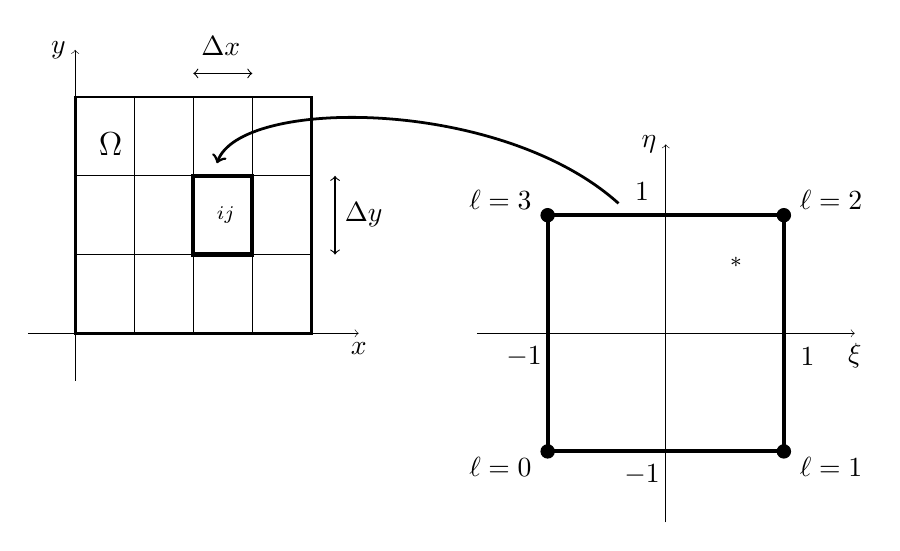
\begin{tikzpicture}[scale=3.0]
% (x,y) elements
  \draw[->,very thin] (-0.2,0.0) -- (1.2,0.0) node[below] {$x$};
  \draw[->,very thin] (0.0,-0.2) -- (0.0,1.2) node[left] {$y$};
  \draw[line width=1.0pt] (0.0,0.0) -- (0.0,1.0) -- (1.0,1.0) -- (1.0,0.0) -- cycle;
  \pgfmathsetmacro\fourth{1.0/4.0}
  \pgfmathsetmacro\third{1.0/3.0}
  \pgfmathsetmacro\twothird{2.0/3.0}
  \draw[xstep=\fourth,ystep=\third,black,thin] (0.0,0.0) grid (1.0,1.0);
  % outline an element
  \draw[line width=1.5pt] (0.5,\third) -- (0.75,\third) -- (0.75,\twothird) -- (0.5,\twothird) -- cycle;
  \node at (0.64,0.5) {$\square_{ij}$};
  \draw[<->] (0.5,1.1) -- (0.75,1.1) node[above,yshift=1mm,xshift=-4mm] {$\Delta x$};
  \draw[<->] (1.1,\third) -- (1.1,\twothird) node[right,yshift=-5mm] {$\Delta y$};
  \node at (0.15,0.8) {\large $\Omega$};

% (xi,eta) reference element
% origin of axes at (2.5,0.0) and square has half-width 0.5
  \draw[->,very thin] (1.7,0.0) -- (3.3,0.0) node[below] {$\xi$};
  \draw[->,very thin] (2.5,-0.8) -- (2.5,0.8) node[left] {$\eta$};
  \draw[line width=1.5pt] (2.0,-0.5) -- (3.0,-0.5) -- (3.0,0.5) -- (2.0,0.5) -- cycle;
  \node at (3.1,-0.1) {$1$};
  \node at (1.9,-0.1) {$-1$};
  \node at (2.4,0.6) {$1$};
  \node at (2.4,-0.6) {$-1$};
  \node at (2.8,0.3) {\large $\square_\ast$};
  \filldraw (2.0,-0.5) circle (0.8pt) node[xshift=-6mm,yshift=-2mm] {$\ell=0$};
  \filldraw (3.0,-0.5) circle (0.8pt) node[xshift=6mm,yshift=-2mm] {$\ell=1$};
  \filldraw (3.0,0.5) circle (0.8pt) node[xshift=6mm,yshift=2mm] {$\ell=2$};
  \filldraw (2.0,0.5) circle (0.8pt) node[xshift=-6mm,yshift=2mm] {$\ell=3$};

% arc
  \draw[->,line width=1.0pt] (2.3,0.55) .. controls (1.8,1.0) and (0.7,1.0) .. (0.6,0.72);
\end{tikzpicture}
\caption{Each element $\square_{ij}$ in the domain $\Omega$, a square in this case, is the image under a map $\left(x(\xi,\eta),y(\xi,\eta)\right)$ of a reference element $\square_\ast = [-1,1]\times[-1,1]$.  The corners of the reference element, and thus of $\square_{ij}$ as well, are locally-numbered $\ell=0,1,2,3$.}
\label{fig:q1grid}
\end{figure}

FIXME hat functions

\begin{equation}
  \psi_{i,j}(x_r,y_s) = \delta_{ir} \delta_{js}  \label{eq:of:phinodewise}
\end{equation}

\begin{equation}
  \psi_\ell(\xi,\eta) = \psi_\ell(x(\xi,\eta),y(\xi,\eta)) = \chi_\ell(\xi,\eta)  \label{eq:of:phionref}
\end{equation}

\begin{equation}
  (\grad \psi_\ell)(\xi,\eta) = \left<FIXME\right>  \label{eq:of:gradphionref}
\end{equation}

\begin{marginfigure}
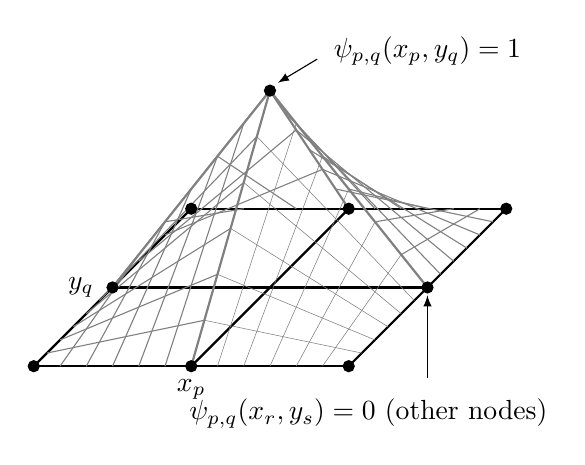
\begin{tikzpicture}[scale=0.5]

  % strong grid around elements
  \draw[thick] (0,0) -- (8,0);
  \draw[thick] (2,2) -- (10,2);
  \draw[thick] (4,4) -- (12,4);
  \draw[thick] (0,0) -- (4,4);
  \draw[thick] (4,0) -- (8,4);
  \draw[thick] (8,0) -- (12,4);

  \def\ytop{7};

  % tent lines
  \draw[gray,thick] (6,\ytop) -- (4,0);
  \draw[gray,thick] (6,\ytop) -- (2,2);
  \draw[gray,thick] (6,\ytop) -- (10,2);
  \draw[gray,thick] (6,\ytop) -- (8,4);

  \def\dx{(10.0-6.0)/6};
  \def\dy{(2.0-\ytop)/6};
  \foreach \jj in {1,...,5}
  {
       \draw[gray,very thin] ({6+\jj*\dx},{\ytop+\jj*\dy}) -- ({4+(4/6)*\jj},0.0);
  }

  \def\dx{(4.0-6.0)/6};
  \def\dy{(0.0-\ytop)/6};
  \foreach \jj in {1,...,5}
  {
       \draw[gray,very thin] ({6+\jj*\dx},{\ytop+\jj*\dy}) -- ({10-(2/6)*\jj},{2-(2/6)*\jj});
  }

  \def\dx{(2.0-6.0)/6};
  \def\dy{(2.0-\ytop)/6};
  \foreach \jj in {1,...,5}
  {
       \draw[gray,thin] ({6+\jj*\dx},{\ytop+\jj*\dy}) -- ({4-(4/6)*\jj},0.0);
  }

  \def\dx{(4.0-6.0)/6};
  \def\dy{(0.0-\ytop)/6};
  \foreach \jj in {1,...,5}
  {
       \draw[gray,thin] ({6+\jj*\dx},{\ytop+\jj*\dy}) -- ({2-(2/6)*\jj},{2-(2/6)*\jj});
  }

  \def\dx{(10.0-6.0)/6};
  \def\dy{(2.0-\ytop)/6};
  \foreach \jj in {1,...,5}
  {
       \draw[gray,thin] ({6+\jj*\dx},{\ytop+\jj*\dy}) -- ({8+(4/6)*\jj},4.0);
  }

  \def\dx{(8.0-6.0)/6};
  \def\dy{(4.0-\ytop)/6};
  \foreach \jj in {1,...,5}
  {
       \draw[gray,thin] ({6+\jj*\dx},{\ytop+\jj*\dy}) -- ({10+(2/6)*\jj},{2+(2/6)*\jj});
  }

  \def\dx{(2.0-6.0)/3};
  \def\dy{(2.0-\ytop)/3};
  \foreach \jj in {1,...,2}  % reduce clutter
  {
       \draw[gray,thin] ({6+\jj*\dx},{\ytop+\jj*\dy}) -- ({8-(4/3)*\jj},4.0);
  }

  \def\dx{(8.0-6.0)/3};
  \def\dy{(4.0-\ytop)/3};
  \foreach \jj in {1,...,2}
  {
       \draw[gray,thin] ({6+\jj*\dx},{\ytop+\jj*\dy}) -- ({2+(2/3)*\jj},{2+(2/3)*\jj});
  }

  % nodes in base plane
  \filldraw (0,0) circle (4pt);
  \filldraw (4,0) circle (4pt);
  \filldraw (8,0) circle (4pt);
  \filldraw (2,2) circle (4pt);
  %\filldraw (6,2) circle (4pt);   % (x_j,y_k) is at (6,2)
  \filldraw (10,2) circle (4pt);
  \filldraw (4,4) circle (4pt);
  \filldraw (8,4) circle (4pt);
  \filldraw (12,4) circle (4pt);

  % node at tent top
  \filldraw (6,\ytop) circle (4pt);

  % annotate
  \draw (10,\ytop+1.0) node {$\psi_{p,q}(x_p,y_q)=1$};
  \draw[-latex] (7.2,\ytop+0.8) -- (6.2,\ytop+0.2);
  \draw (8.5,-1.2) node {$\psi_{p,q}(x_r,y_s)=0$ (other nodes)};
  \draw[-latex] (10,-0.3) -- (10,1.8);

  % label center point
  \draw (4,-0.6) node {$x_p$};
  \draw (1.2,2) node {$y_q$};

\end{tikzpicture}

\caption{FIXME}
\label{fig:q1hat}
\end{marginfigure}


\section{Implementation with objective only}

FIXME code uses \texttt{SNESSetObjective()} only, though also \texttt{SNESSetFunction()}; no hand-made Jacobian at all

FIXME try NCG

\cinputpart{plap.c}{\CODELOC}{FIXME I}{I}{//STARTCONFIGURE}{//ENDCONFIGURE}{code:plapI}

\cinputpart{plap.c}{\CODELOC}{FIXME II}{II}{//STARTEXACTF}{//ENDEXACTF}{code:plapII}

\cinputpart{plap.c}{\CODELOC}{FIXME III}{III}{//STARTOBJECTIVE}{//ENDOBJECTIVE}{code:plapIII}

\cinputpart{plap.c}{\CODELOC}{FIXME IV}{IV}{//STARTMAIN}{//ENDMAIN}{code:plapIV}


\section{Residual function $=$ gradient}

\cinputpart{plap.c}{\CODELOC}{FIXME V}{V}{//STARTFUNCTION}{//ENDFUNCTION}{code:plapV}


\section{Exercises}

\renewcommand{\labelenumi}{\arabic{chapter}.\arabic{enumi}\quad}
\renewcommand{\labelenumii}{(\alph{enumii})}
\begin{enumerate}
\item Prove coercivity \eqref{eq:of:coercivity} and convexity \eqref{eq:of:convexity} of functional $I[u]$ defined in \eqref{eq:of:functional}.  The finite dimensional facts that FIXME for $\xi,\eta\in\RR^n$ will be useful.
\item FIXME
\end{enumerate}